\documentclass[a4paper,11pt]{scrreprt}

\usepackage[utf8]{inputenc}
\usepackage[ngerman]{babel}
\usepackage[T1]{fontenc}
\usepackage{graphicx}
\usepackage{hyperref}
\usepackage{listings}
\usepackage{url}
\usepackage{bm}


\bibliographystyle{unsrt}

\title{Projektarbeit \\ Konfigurierbare Formulare}
\subtitle{Informatikprojekt \\ Hochschule Ravensburg-Weingarten}
\author{Arthur Becker}
\date{15. April 2021}
\setcounter{secnumdepth}{5}
\setcounter{tocdepth}{5}

%\pagestyle{headings}

\usepackage{fancyhdr}
\pagestyle{fancy}


%
\lhead{\slshape \rightmark}
\chead{}
\rhead{}
%%
\lfoot{}
\cfoot{\thepage}
\rfoot{}
%%
\renewcommand{\headrulewidth}{0.4pt}
\renewcommand{\footrulewidth}{0pt}

\begin{document}

\maketitle

\chapter{Zusammenfassung}
Das Ergebnis dieser Arbeit zeigt, wie man Formularkomponente dynamisch erzeugen kann. 
Häufig werden Formulare statisch in Projekten eingesetzt. Das bedeutet, dass diese eine feste Struktur haben und bei jedem Aufruf identisch gerendert werden. Für viele Verwendungsfälle reicht das auch aus. Jedoch nicht für alle Fälle. Möchte man Formularkomponente die sich beispielsweise an Input Daten ausrichten, muss ein anderer Ansatz verwendet werden. In diesem Projekt ist eine Komponente geschrieben, die basierend auf den Input Daten entsprechende Formularelemente rendert. Somit kann während der Laufzeit je nachdem was für Input Daten geladen werden eine Komponente erstellt werden, die sich von den anderen unterscheidet. Zusätzlich kann man die Input-Daten, die geladen werden, auch noch nachträglich ändern, was zu einer noch größeren Flexibilität führt.

  


\tableofcontents
\newpage

\chapter{Motivation}
Die Motivation beruht auf dem Wunsch eine Webapp zu schreiben, mit der man Prozesse modellieren kann. Zwar gibt es auf dem Markt den ein oder anderen Vertreter, jedoch immer mit einem Haken verknüpft. Entweder benötigt man ein bestimmtes Betriebssystem oder man kann im Nachhinein ein Prozess oder eine ganze Prozesskette nicht mehr verändern. 
Der erste Schritt für eine solche Prozessmodellierung stellt das Erstellen von konfigurierbaren Formularkomponenten dar. Das Erstellen von Komponenten abhängig von den Input-Daten ermöglicht das Modellieren der verschiedensten Prozesse. 
Dies stellt eine grundlegende Basis dar, auf der nachfolgende Schritte arbeiten können. 



\chapter{Grundlagen}



\section{Konfigurierbare Formulare}
Das sind Formulare, die basierend auf der Struktur einer JSON File erstellt werden. Sowie die Daten in der JSON File sich unterscheiden können, so unterscheiden sich auch die daraus erstellten Formulare.


\section{Node.js}
Mit NodeJS kann man einfache Kommandozeilenwerkzeuge schreiben oder auch
komplexere Webanwendungen. Da NodeJS auf der Javascript Chrome V8 Engine basiert
ermöglicht es den Programmierern das Schreiben der Serveranwendung (Backend) in
Javascript. \cite{Weiss2019}

\section{Express}
“Schnelles, offenes, unkompliziertes Web-Framework für Node.js” \cite{None2019}

\section{React}
React ist eine Frontend Bibliothek, die es dem Programmier ermöglicht eine moderne Webseite zu programmieren. 
Gerade für Single Page Applications wird React häufig verwendet. Im Gegensatz zu anderen Frameworks, gibt es in React keine proprietäre Kommandos die gelernt werden muss. Hier wird mit JavaScript und der Erweiterung Es6 gearbeitet. 


\section{UUID}
UUID steht für Universally Unique Identifier. Auch als GUID bekannt (Globally Unique Identifier). Diese ID ist 128 bit groß und garantiert globale Einzigartigkeit. \cite{rfc4122} Damit kann sichergestellt werden, dass Komponente die eine ID zugewiesen bekommen haben, immer eindeutig ansprechbar sind.

\section{MobX}
Um States zu verwalten wird MobX eingesetzt. Verändern sich States wird die Komponente, in denen sich diese States befinden, neu gerendert. Sollen Komponente auf States hören die außerhalb des eigenen Wirkungsbereichs liegen, benutzt man einen Store. In diesen Stores werden die States und die Funktionen, die diese States manipulieren, definiert. Über das Pattern Observable, können die Komponente als Observer, die observable States observieren. Bei Veränderungen dieser States reagieren die Komponenten, die diese States implementiert haben, sofort und triggern die Render Funktion. 





\chapter{Problem und Anforderungsanalyse}
Formularkomponente haben meist einen festgelegten Aufbau, der sich ohne weiteren Programmieraufwand nicht verändert. Bei Fällen, in denen man die gleichen Daten eines Users benötigt, wie zum Beispiel in Registrierungen, ist dieser Ansatz erfolgreich. Bei Formularen, bei denen die Anzahl der Formularelemente abhängig von bestimmten Daten ist, stößt der statische Ansatz auf seine Grenzen. Aus diesem Grund ist das Erstellen von konfigurierbaren Formularen eine Notwendigkeit. Da dadurch Use Cases abgedeckt werden, bei denen der Aufbau der Formularkomponenten abhängig von Eingabedaten ist. Als Beispiel kann man Prozesse abbilden, die sich vom inneren Aufbau ändern, je nachdem welche Input-Daten eingegeben werden.  


\section{Musskriterien}
\subsection{konfigurierbare Formulare}
Formulare sollen konfigurierbar gemacht werden. Über Eingabe Daten werden diese Formulare konfiguriert und dementsprechend gerendert.
\subsection{Aktualisierbar}
Diese Formulare können auch im Nachhinein in der Webapp verändert werden.
\subsection{Über JSON Files erstellbar}
Aus einer Datenquelle wird eine JSON geladen, die einem festgelegten Format folgt. Der Anwender kann diese JSON File nutzen um ein Formular zu erstellen. 
\subsection{Eingabemöglichkeit schaffen}
Über die Webapp kann der User eine JSON File erstellen. Diese wird dann sogleich für das Formular verwendet.

\section{Wunschkriterien}
\subsection{Ordentliche Darstellung}
Die optische Darstellung soll simpel und gut visuell aussehen.
\subsection{Übersicht}
Eine Übersicht schaffen in der alle Formulare einsehbar sind. 
 

\chapter{Lösungsvorschläge}
\section{Datenbank}
Für die Speicherung der JSON Files wird eine Datenbank benötigt. Damit der gesamte Komplex auf jeglicher Plattform aufgebaut werden kann, wird eine Datenbank benötigt die auf allen relevanten Systemen läuft. Weiter ist es wichtig eine DB auszuwählen, die jahrelang unterstützt wird und sich auch bewiesen hat. Damit stehen zur Auswahl MySQL, PostgreSQL und MongoDB. Um zuverlässig Daten abzuspeichern und ohne Komplikationen eine Verbindung zum Node.js Server aufzubauen, ist eine dieser Datenbanken eine gute Option. 


\section{Web- und UI Framework}
In der Webentwicklung gibt es viele Frameworks die für die verschiedensten Use Cases geeignet sind. Für die Entwicklung von Single Page Applications ist die Wahl zwischen Angular, Vue.js und React. Da die Erfahrung nur bei React liegt, ist die Wahrscheinlichkeit hoch das React verwendet wird. Zudem bietet React ordentliche UI Frameworks an, die vom Design als auch von der Dokumentation eine Qualität versprechen. Hier stehen Semantic UI und Material UI zur Wahl.


\section{Backend}
Da genügend Erfahrung mit Node.js vorhanden ist, wird für dieses Projekt Node.js in Verbindung mit dem Framework Express.js verwendet. 



\chapter{Auswahl der Lösungen anhand der Anforderungen}

\section{Datenbank}
Damit die Daten sicher und ohne Komplikationen gespeichert werden können braucht man eine zuverlässige Datenbank. MySQL ist eine bewährte Datenbank, die den Anforderungen, ob  zuverlässiges speichern oder anbieten von verschiedenen Datentypen genügt. Zudem ist ein wichtiger Entscheidungsfaktor die Möglichkeit über Sequelize die Datenbank mit Node.js zu verknüpfen. 

\section{Webapp}
Als Frontend Framework wird React eingesetzt. Einerseits, weil genügend Erfahrung mit diesem Framework vorhanden ist und andererseits weil es den Anforderungen genügt. 
React verwendet als Sprache hauptsächlich JavaScript. Mit JS kann mittels der Fetch Methode von Backend Systemen beziehungsweise APIs Daten laden. Bedeutet, man ist in der Lage JSON Dateien, die für die Konfiguration der Formulare eingesetzt werden, einfach vom Server zu beziehen. Zudem bietet die Sprache die Möglichkeit mit JSON Files umzugehen. Weiter wird JSX unterstützt. Das hilft in JavaScript mit Tags zu arbeiten. Dynamisches laden von bestimmten Tags wird somit unterstützt. 


Für das Design der Webseite ist der Einsatz eines Design-Templates, wie z.B. Semantic-UI
hilfreich. Da dadurch eine gute Darstellung ermöglicht wird. 
Die Dokumentation auf der Webseite von Semantic-UI ist verständlich und
bietet mit Code Beispielen eine gute Unterstützung.
\\
\section{Backend}
Damit der Fokus auf das eigentliche Projekt gelegt werden kann, wird ein Server verwendet, bei dem Erfahrung vorhanden ist. Es wird ein Node.js Server in Kombination mit Express verwendet. Zudem hat Node.js eine große Funktionsfähigkeit, dank der großen Menge an Modulen, die einfach integriert werden können. Als Beispiel hierfür ist Sequelize zu nennen, mit dem man qualitativ auf die Datenbanktabellen Zugriff hat. So ist die Manipulation von Daten einfach zu realisieren. Mit diesen Technologien kann schnell und einfach eine API erstellt werden die den Anforderungen genügt.

\chapter{Umsetzung}
\section{Home}
Gestartet wird mit der Home Seite. Zunächst benötigt man nur einen Button, der einen Modal aufruft, um dem User die Wahl zwischen zwei Optionen zu bieten. Die Callbackfunktion, die dabei aufgerufen wird, öffnet das Modal. 
\begin{lstlisting}
<Button circular icon='plus'  style={spacing} primary
onClick={this.onClickPlusBtn.bind(this)} />
\end{lstlisting}
\begin{figure}[ht]
\centering
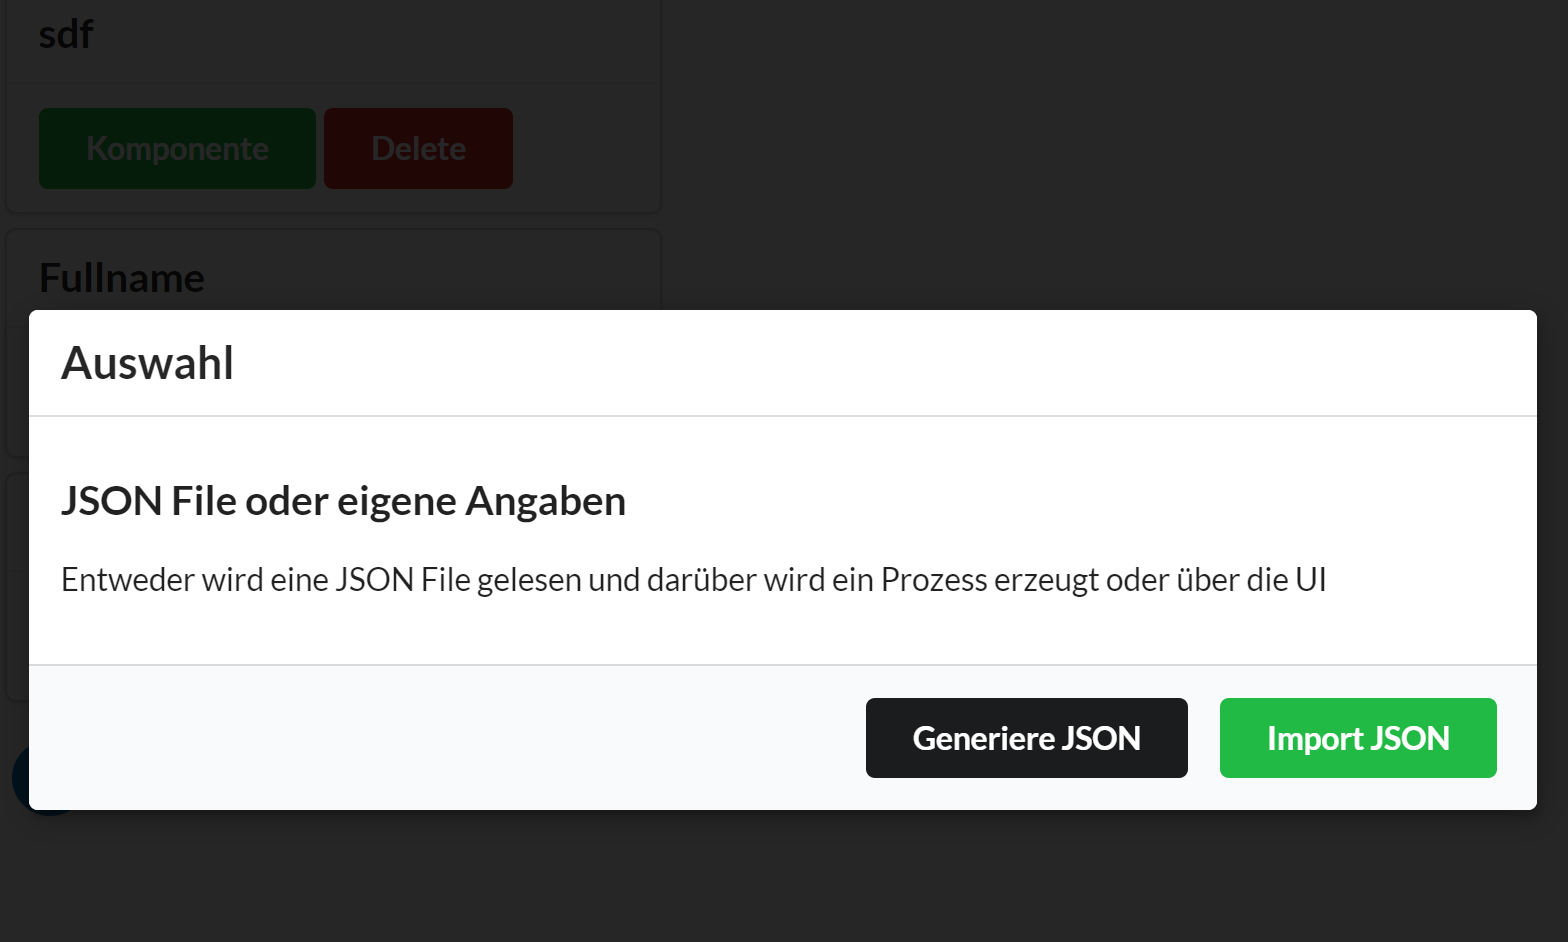
\includegraphics[width=10cm]{Pictures/Modal.png}
\caption{Modal}
\label{Modal}
\end{figure}
\hfill \break
Der nächste Schritt ist, den Buttons im Modal ebenso Callbackfunktionen mitzugeben. Der eine führt durch das Klicken auf den Generiere JSON Button den User zum Pfad /model, während der andere Button den User zum Pfad /jsonfiles führt. Sind diese Funktionen implementiert, ist der nächste Schritt das Programmieren der View, mit der man JSON modelliert. 
\hfill \break
\hfill \break
\hfill \break
\hfill \break
\section{JSON-Modellierung}
Die Idee ist eine Box zu erstellen, in der ein Dropdown, ein Input-Feld, ein Slider, nur beim Input, und ein Hinzufügen sowie ein Entfernen Button als Bedienelemente zur Verfügung stehen. Damit man auch den Namen des Prozesses eingeben kann, wird noch eine kleine Box mit einem Input-Feld an oberster Stelle gerendert. 
\begin{figure}[ht]
\centering
\includegraphics[width=10cm]{Pictures/Model2.png}
\caption{JSON Bildung über Boxen}
\label{JSON Bildung über Boxen}
\end{figure}
\hfill \break
Der Datentyp kann über den Dropdown ausgewählt werden. Über den Input, der abhängig ist vom Datentyp, kann man entweder Text, Zahlen, Boolean oder weitere Angaben wie Zeit oder Datum eingeben. Das Verstellen des Sliders bewirkt, dass der Datentyp und das vom User Eingetragene in die Outputbox kopiert wird. Bedeutet, es soll das, was als Input kommt, auch als Output wieder herausgehen. Zu guter Letzt haben die Buttons den Zweck,  eine Box-Komponente zu erstellen oder zu entfernen. Das bedeutet man kann unzählige Inputs sowie Outputs erstellen. Somit kann man verschiedenste Prozesse die allerlei Inputs und Outputs haben modellieren.
\\
Da die Darstellung soweit fertig ist, ist die Logik der nächste Schritt. Als Erstes wird dem Dropdown eine onChange mitgegeben, die wie folgt aussieht. 
\begin{lstlisting}
 onChangeInputSelection (a,b) {
   this.Input.forEach(item => {
    if(b.id === item.idInputArr[0].dropDownId){
      item.datatype = b.value;
      console.log(item.datatype);
      this.setState({
        dummyDatatype : b.value
      });
      this.simpleBoolean = true;
    }
   });
\end{lstlisting}
this.Input ist ein Array, das die Daten der Boxen speichert. Mittels der Foreach Schleife iteriert man durch dieses Array. Das Ziel dabei ist es, das Element zu finden, dass dieselbe Id hat wie die vom Dropdown, die den Callback ausgelöst hat. Beim passenden Datensatz wird nun der Datentyp auf den Wert der sich in b.value verbirgt geändert. Das neu Setzen der State Dummy Variable hat folgende Gründe. Zuerst muss neu gerendert werden, damit die Veränderung im Dropdown zusehen ist, zudem wird eine Voreinstellung für die nächste Box erstellt. Heißt, wird über den Plus Button eine neue Box erstellt, ist der Datentyp der, der zuletzt eingestellt wurde.
\\
So ähnlich sieht es auch bei den Input-Feldern aus. Die Input-Felder erhalten eine onClick Callback Methode. Mit dieser ruft man eine Methode auf die genau wie beim Dropdown durch die Array-Variable this.Input iteriert, nach derselben ID schaut und beim Fund den richtigen Datensatz mit dem neuen Wert aktualisiert. 
\\
Als Nächstes wird das Hinzufügen von neuen Boxen behandelt. Hier muss man eine neue Box erstellen. Wichtig hierbei ist es, jedem Element eine ID mitzugeben damit man später bei Callback Funktionen auf die richtigen Elemente reagieren kann. Um die Arbeit zu erleichtern wird hier das Paket UUID-React verwendet. Dieses Paket liefert eine Funktion die eine eindeutige ID zurückliefert. 
\begin{lstlisting}
const dropDownId = uuid()
\end{lstlisting}
Bevor die Box erstellt wird, muss geklärt werden, ob die zu erstellende Box, die erste ist. 
Wenn es das erste Element ist, soll eine Box erstellt werden, die kein Minus Button hat.
Da sonst die Boxen komplett verschwinden könnten und somit kein passendes JSON File erstellt werden könnte.  Hierfür wird der State-Array NewInputArray herangezogen. Hier befinden sich die Komponenten. Ist dieser leer, bedeutet es, dass dieser, eine Box erstellen muss, die kein Minus Button verfügt. Sind in dem Array schon Boxen drin, wird eine Komponente erstellt mit Minus Button. Was in der Abbildung 7.2 dargestellt wird.  
Beim Erstellen der Box fügt man diese Box in die State-Variable NewInputArray hinzu und die ID Daten in die this.Input Array.
 
\\
Beim Minus Button also dem Entfernen der Boxen, ist es wichtig darauf zu achten, dass man aus den beiden Arrays die Daten entfernt. Dies kann man gut über die Funktion Filter ausführen. Elemente, die nicht diese ID haben, werden zunächst in ein separates Array gespeichert und anschließend werden diese temporären Arrays herangezogen um die Arrays this.Input und this.state.NewInputArray neu zu befüllen.
Damit kann man aus der NewInputState Variable als auch in der this.Input Variable die Komponenten und Daten entfernen, die nicht mehr benötigt werden.
\hfill \break
\hfill \break
\hfill \break
\hfill \break
\begin{lstlisting}
let newArr = this.state.NewInputArray.filter(item => (
      (item.props.btnMinusId !== b.id)
    ));
    console.log(this.Input);
    this.Input = this.Input.filter(item => (
      (item.idInputArr[4].btnMinusId !== b.id)
    ));
    console.log(this.Input);
    this.setState({ NewInputArray: newArr })
\end{lstlisting}

Bei der Implementierung der Callback Methode für den Radio Slider müssen 4 Fälle beachtet werden. Doch zunächst wird über die ID überprüft, welche Komponentenbox den Radio Slider aktiviert hat. Dadurch werden die richtigen Komponenten angesprochen und es werden die Daten vom Input in Variablen gelagert. 
\begin{lstlisting}
this.Input.forEach(item => {
    if(b.id === item.idInputArr[2].radioId){
      item.isEdit = !item.isEdit;
      key = b.id;
      tmpDatatype = item.datatype;
      tmpInput = item.input;
\end{lstlisting}
Der erste Fall ist, wenn die erste Komponentenbox den Radio Slider aktiviert. 
Zunächst wird durch NewOutputArray iteriert. Das Ziel davon ist, die Komponente anzusprechen die, die gleiche ID hat wie die in der Radio Slider ID. Damit wird sichergestellt, dass wenn mehrere Output-Boxen vorhanden sind, diese nicht angesprochen werden. Mittels unshift wird die neue Output-Box, die jetzt beim DropDown und beim Inputfeld disabled sind, in diese temporäre Array-Variable gespeichert und mit Hilfe der this.setState wird der eigentliche Array, der die Boxen darstellt, aktualisiert. Am Ende werden noch die Daten in ein Objekt gespeichert und in die erste Position des this.Output Arrays hinzugefügt. 
So hat man die Darstellung, sowie die Daten aktualisiert.

\begin{lstlisting}
if(item.isEdit === true){
        isDisabled = true;
        if(item.isFirst === true){
          
          this.state.NewOutputArray.forEach(itemNewOutput => {
            if(itemNewOutput.key === b.id){
              dropDownId = itemNewOutput.props.dropDownId;
              formInputId = itemNewOutput.props.formInputId;
              btnPlusId = itemNewOutput.props.btnPlusId;
              btnMinusId = itemNewOutput.props.btnMinusId;
            }else if(itemNewOutput !== b.id &&
            this.state.NewInputArray.length > 1){
              arr.push(itemNewOutput);
            }
          });
          arr.unshift(this.updateOutput(key,
          dropDownId, formInputId,btnPlusId,
          btnMinusId, item.isFirst, tmpDatatype,
          isDisabled));
          this.setState({
            NewOutputArray : arr
          });
          let idArr = [{dropDownId : dropDownId},
          {formInputId: formInputId},
          {btnPlusId : btnPlusId},
          {btnMinusId : btnMinusId}
          ,{radioId : b.id}]
          let obj = {idOutputArr : idArr,
          input : tmpInput, datatype : tmpDatatype,
          id : uuid(), data : "", isEdit : true};
          this.Output[0] = obj;
\end{lstlisting}
Ist die Komponente nicht die erste, wird der zweite Fall behandelt. Beim zweiten Fall wird eine neue Output-Box erstellt und in die NewOutputArray Variable hinzugefügt. Wichtig dabei ist, dass die Komponenten-Elemente alle eine neue ID bekommen, bis auf RadioSlider ID. Hier wird die ID von der Input-Box Radio Slider verwendet. Diese ID wird für Fall 4 eingesetzt. Bei den Fällen 3 und 4 geht es um das Ausschalten des Radio Sliders.
Wird der Radio Slider ausgeschaltet, wird überprüft, ob das erste Element dies ausgeführt hat oder nicht. Führt das erste Element diese Aktion aus, wird alles sowie in Fall 1 ausgeführt bis auf einen Aspekt. Der DropDown und das Inputfeld werden nicht mehr aus Disabled geschaltet, da diese Output-Box nicht mehr mit der Input-Box in Abhängigkeit steht. 
Wird nicht die erste Komponente ausgeschaltet, wird Fall 4 behandelt. Das Ergebnis hiervon ist, dass Entfernen der Output-Box. Hier wird wie in Fall 1 durch die NewOutputArray iteriert. Ist eine Komponente vorhanden mit der gleichen ID, wird diese entfernt. Damit auch die Daten verschwinden wird mit der Filter Methode durch die this.Output iteriert. 
\begin{lstlisting}
this.Output = this.Output.filter(obj => (
            (obj.idOutputArr[4].radioId !== b.id))
          );
\end{lstlisting}




Zu guter Letzt haben wir den Button für die Bestätigung. 
Wichtig hierbei ist der Inhalt der Callback Methode, die beim Klick aufgerufen wird.
\begin{lstlisting}
this.createProzessJSON = {name : this.prozessName, 
prozessId : uuid(),
InputArr : this.Input, 
OutputArr : this.Output}
modellierStore.setDieProzess(this.createProzessJSON);
window.location.hash = '/innercomp';
\end{lstlisting}
Hier wird ein Objekt erstellt der den Prozessnamen, die Input-Daten sowie die Output-Daten speichert. Dieser wird für die Erstellung der Formulare verwendet.
Damit man diesen Prozess bei anderen Views auch verwenden kann, wird ein Store implementiert, der über eine dort definierte Variable dieses Objekt aufnimmt. 
Wird dieser Store in einer Komponente importiert, kann man die dort definierten Methoden und Variablen benutzen. Ein weiterer Vorteil davon ist, dass wenn so eine Variable in der Render sich befindet und diese sich aktualisiert, wird die Render Methode neu aufgerufen, damit neu gerendert wird. 



\section{Ergebnis}
Bevor man die JSON-Datei erstellt, erhält man über diese View noch eine Übersicht. 
Klickt man im Navigationsbar auf Home, wird der Prozess verworfen. Ist man mit dem Prozess zufrieden, kann man über Bestätigen den Prozess speichern, indem aus dem Objekt ein JSON wird und dieser in die Datenbank transferiert und gespeichert wird. 
Um die Daten anzuzeigen wird erst einmal die Variable aus dem Modellierstore importiert. 
Mittels der ES6 Spread Methode kann man auf die einzelnen Variablen zugreifen. In dem man mit der Foreach durch die Input und Output Arrays iteriert, holt man jede hinzugefügte Input und Output Information. 
Diese Daten werden in den Klassen Member gespeichert. Die UI Elemente beziehen ihre Informationen aus diesen Membervariablen. 

\begin{figure}[ht]
\centering
\includegraphics[width=12cm]{Pictures/result.png}
\caption{Overview der eingegebenen Daten}
\label{JSON Bildung über Boxen}
\end{figure}
\hfill \break

\section{Mit der Komponente interagieren}

Über die Fetch Methode werden die JSON-Daten, die man über die Webapp in der Ergebnis-View bestätigt hat, aus der Datenbank geholt. Bevor man aus diesen Daten ein Formular erstellen kann, muss eine Interaktionsmöglichkeit geschaffen werden. 
In der Home wird durch die JSON Files iteriert und alle Daten werden in Cards geschrieben. Klickt man auf diese Card, kommt auf eine neue View, die es dem User erlaubt mit dem Formular zu interagieren.
\begin{figure}[ht]
\centering
\includegraphics[width=12cm]{Pictures/Prozess_Cards.png}
\caption{Cards für die Interaktion}
\label{JSON Bildung über Boxen}
\end{figure}
\hfill \break

Bei der Darstellung der Formular-Komponenten war Folgendes geplant. 
Inputs werden so wie sie eingetragen wurden angezeigt. Bedeutet, dass keine Interaktion möglich ist, sondern nur die Darstellung dessen was eingegeben wurde. Die andere Möglichkeit ist, wenn ein Input auch als Output aufgefasst wird. Da hat man die Möglichkeit, über die Editierung ein Formular zu erstellen, das einem ermöglicht damit zu interagieren.
\hfill \break
\hfill \break
Beim Klicken des Cards, wie in Abbildung 7.4 zu sehen ist, wird die MobX Variable dieProzesse gefüllt. Über Iterationsprozesse durch diese Variable, werden die Daten in lokale Variablen überführt. 
Damit entschieden werden kann, was genau gerendert werden soll, wird der Datentyp verwendet. 
\begin{lstlisting}
Card_Content (prozName,inputName,id,datatype) {
  let formContent;
  if(datatype === "string"){
    formContent = <Edit key={uuid()}
    prozessName={prozName}
    inputName={inputName}
    id={id}
    onChangeFunction={this.onChangeEdit.bind(this)}
    onChangeCallFunction={this.onChangeCallFunction.bind(this)} />
\end{lstlisting}
\begin{figure}[ht]
\centering
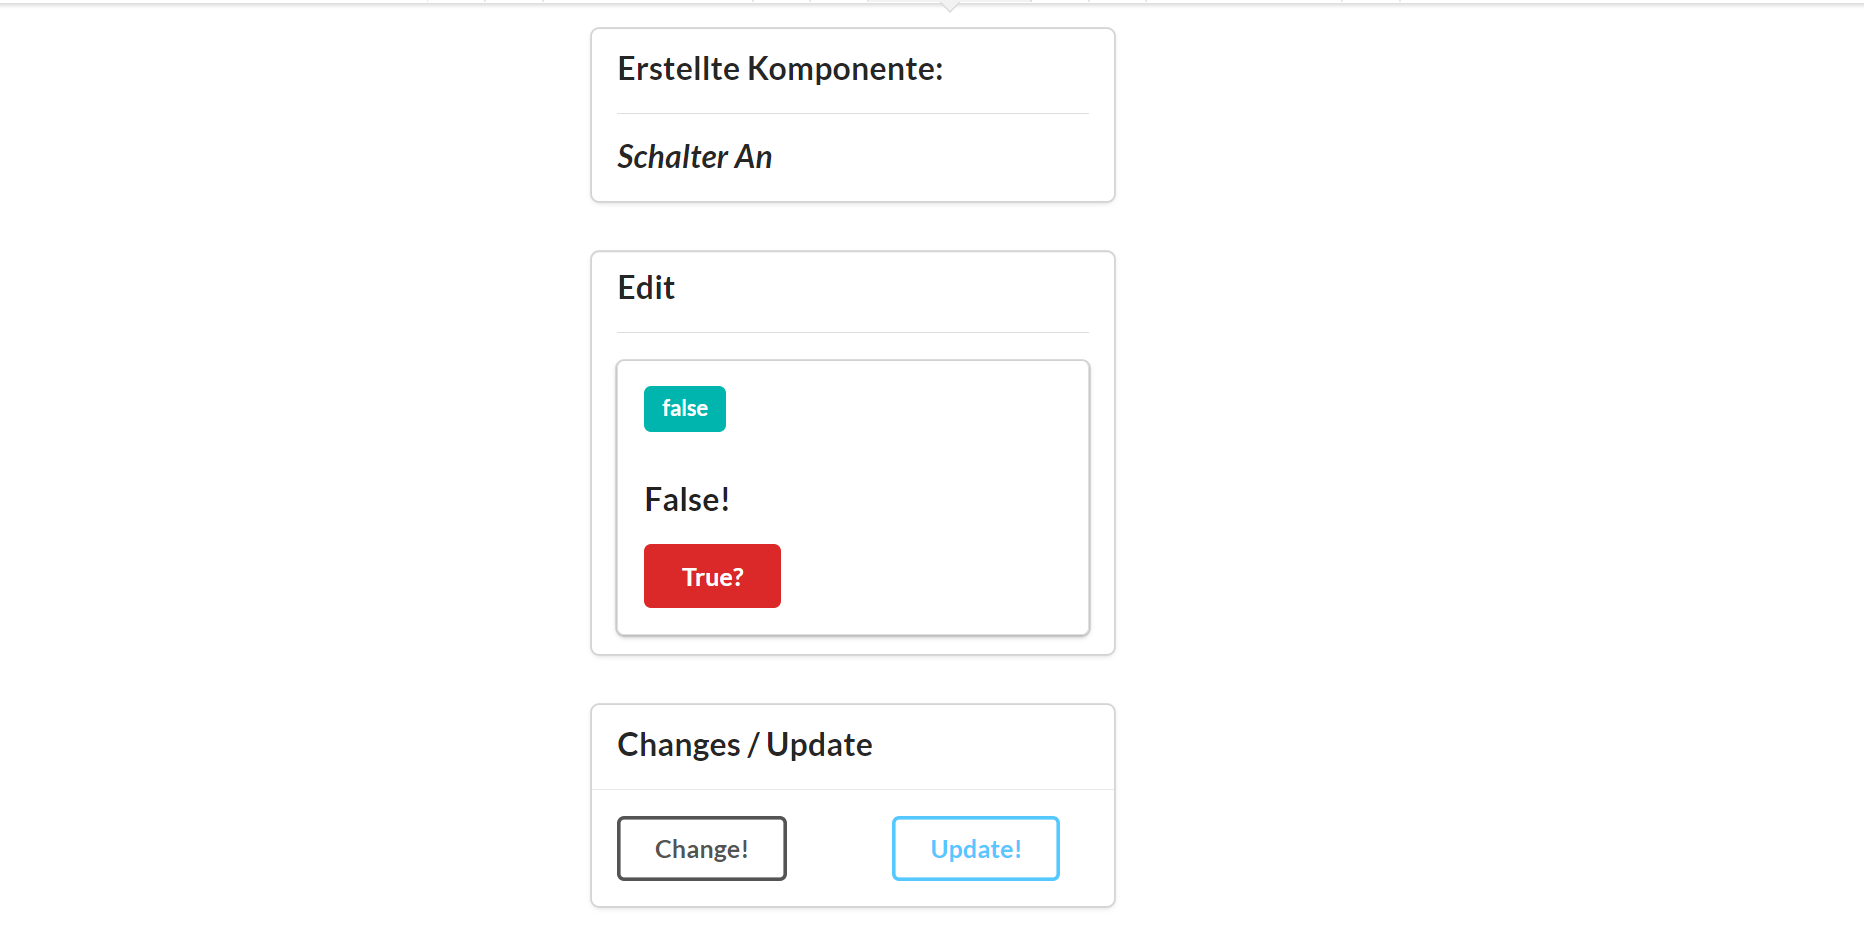
\includegraphics[width=12cm]{Pictures/_schalter.png}
\caption{Interaktion über einen Button}
\label{JSON Bildung über Boxen}
\end{figure}
\hfill \break
Die Anzahl der zu gerenderten Komponenten wird von der Anzahl der definierten Inputs bestimmt. Auf dieser View kann der User nun interagieren. Wie in Abbildung 7.5 zu sehen ist, kann er den Button klicken und den Zustand von False auf True setzen. 

Beim Change Button kommt man auf eine View, die man schon bei der Modellierung zu sehen konnte. Hier kann man, eventuelle Fehler korrigieren. Wenn man noch weitere Inputs und Outputs zu diesem Prozess hinzufügen möchte, kann man dies hier machen. Auch der Prozessname kann wieder verändert werden. 
Im Code hat sich nur eine Kleinigkeit getan. 
\begin{lstlisting}
        inputArr.forEach(item => {
          if(count === 0){
            isFirst = true;
          }else{
            isFirst = false;
          }
          let _item = [...item.idInputArr];
          newInputArr.push(this.updateInput(uuid(),
          _item[0].dropDownId, _item[1].formInputId,
          _item[2].radioId, _item[3].btnPlusId,
          _item[4].btnMinusId, isFirst, item.datatype,
          item.input, item.isEdit));
          this.Input.push(item);
          count++;
        });
        this.changeArrayState(newInputArr,"input");
        count = 0;
        let isFirst = false;
        outputArr.forEach(item => {
          if(count === 0){
            isFirst = true;
          }else{
            isFirst = false;
          }
          let isDisabled = item.isEdit;
          let _item = [...item.idOutputArr];
          newOutputArr.push(this.updateOutput(_item[4].radioId,
          _item[0].dropDownId,
          _item[1].formInputId,_item[2].btnPlusId,
          _item[3].btnMinusId, isFirst, item.datatype,
          isDisabled, item.input));
          this.Output.push(item);
          count++;
        });
        this.setState({
          NewOutputArray : newOutputArr
        });
        this.changeArrayState(newOutputArr,"output");
      }
    }
\end{lstlisting}
Es werden IDs erstellt damit man weiterhin die Verbindung von Komponente und Daten hat. So kann man weiterhin interagieren wie schon auch bei der ersten Modellierungs View. 

Ist man fertig kann man über Update die Veränderungen bestätigen. Hier erscheint die View Result. Hier werden nochmal alle Daten angezeigt. Ist man zufrieden kann man über Bestätigen die Daten speichern. Der einzige Unterschied hier ist, dass diesmal keine Add Methode sonderen eine Update Methode ausgeführt wird. Da der bestehende Datensatz nur aktualisiert werden muss. Durch die ID wird erkannt um welchen Datensatz es sich handelt. Im Backend wird dann Update aufgerufen. Da dies im Kapitel Backend näher ausgeführt ist, sei hier nur gesagt, dass durch die SQL Where Klausel der richtige Datensatz ausgewählt wird, mit den neuen Datensatz aktualisiert und wieder in die DB geschrieben wird. 


\section{JSON Files erstellen und hochladen}
Wie in der Anforderung beschrieben, sollen auch aus schon bestehenden JSON Files Formularkomponenten erstellt werden. Damit dies funktionieren kann, brauchen die JSON-Files eine festgelegte Struktur. 
\hfill \break
\hfill \break
\hfill \break
\hfill \break
\begin{lstlisting}
{
        "id" : 326632,
        "name" : "Prozess JSON_from_Db",
        "inputArr" : [
            {
                "idInputArr" : 321,
                "input" : "Test",
                "datatype" : "text",
                "isEdit" : false,
                "editing" : " ",
                "id" : 1234
            },
            {
                "idInputArr" : 123,
                "input" : "10",
                "datatype" : "number",
                "isEdit" : true,
                "editing" : "",
                "id" : 4321
            }
        ],
        "outputArr" : [
            {
                "idOutputArr" : 555,
                "input" : "isOkay",
                "datatype" : "bool",
                "id" : 4321,
                "data" : ""
            }
        ]
}
\end{lstlisting}
In diesem Stil soll ein JSON Konstrukt aussehen, damit ohne Komplikationen ein Formular erstellt werden kann. Ein Aspekt der beleuchtet werden muss ist die Option isEdit. isEdit ist eine Boolean Variable die aussagt, ob die Input-Daten auch als Output-Daten verwendet werden dürfen. In der Webapp wird dies über den Radio Slider, der in der Box integriert ist, ausgeführt. Wird der Slider eingeschaltet, werden die Daten, die aus der Input Box stammen in das Objekt des Outputs geschrieben. Das muss bei der manuellen Erstellung solcher JSON Files beachtet werden, da ansonsten keine passenden Output-Daten vorhanden sind, obwohl isEdit auf true gesetzt ist. Zwar wird die Webapp einen Fehler ausgeben, dennoch sollte das, wenn möglich, vermieden werden. 
\hfill \break
\hfill \break
\hfill \break
\hfill \break
Die Webapp lädt über die Fetch Funktion, die im Abschnitt Backend näher beleuchtet ist, diese JSON Files. Im Bereich Home wo man über den Plus Button das Modal aufruft, wird jetzt der zweite Button definiert. Hier wird nur ein Callback hinzugefügt, der den Zweck hat, den User zum Pfad /jsonfiles zu befördern. 
Damit man so ein JSON File nutzen kann, muss man dem User eine Bedienmöglichkeit geben. Für jedes JSON File gibt es einen entsprechenden Button. Klickt man auf diesen werden alle Informationen die in dem JSON File vorhanden sind genutzt, um eine Komponente zu erstellen.

Damit dies funktioniert, muss man zunächst vom Modellierstore die Variable allCreateProzesses in die JSON-File Page importieren. Da dies ein MobX Array ist, muss zunächst über die ES6 Spread Methode, die sich darin befindenden Daten, in eine separate Variable laden. Nun iteriert man durch diese neue Variable. Für jede JSON File wird ein Button erstellt. Der Name des JSON Files wird zur Beschriftung des Buttons verwendet. 
Zudem hat der Button auch die ID, die in der JSON aufgeführt ist. 
\begin{figure}[ht]
\centering
\includegraphics[width=12cm]{Pictures/json_File.png}
\caption{Json Files aus der DB mit denen man interagieren kann}
\label{JSON Files aus der Datenbank}
\end{figure}
\hfill \break

Beim Klick des Buttons wird eine Callback Methode aufgerufen. In dieser Methode wird durch this.Prozesse, wo alle JSON Files nochmal hinterlegt sind, iteriert und wenn die ID des Buttons mit der ID eines JSON File Prozesses übereinstimmt, werden die Daten in ein Objekt hinzugefügt. Dieses Objekt wird dann zum neuen DieProzess, die Variable die verwendet wird, um die kumulierten Daten von einer View zur nächsten zu transportieren. Da die Struktur sich nicht groß von der manuell erstellten Version unterscheidet, muss nichts weiter getan werden. Die Daten werden gelesen und die richtigen Komponenten werden ausgesucht. Somit hat man dann ein Formular über ein JSON File erstellt. 


\section{Backend}
In der App.js werden Routen festgelegt. Damit die Prozessdaten Input und Output in der Datenbank festgehalten werden können, muss man eine Verbindung zu der Datenbank schaffen. Hierfür wird Sequelize eingesetzt. 
Man erstellt sich eine Variable die alle wichtigen Daten für die Datenbank bereitstellt. Also welche Datenbank angesprochen wird, welcher Username verwendet wird und welches Passwort dazugehört. 
Als Nächstes wird die authenticate eingesetzt, um die Verbindung zur Datenbank aufzubauen.
 \begin{lstlisting}
var sequelize = require('sequelize');

var sequelizeInstance = new sequelize('Prozesse', 'arthur', 'passwd', {
    host: '192.168.0.90',
    port: 3306,
    dialect: 'mysql'
    
});

sequelizeInstance.authenticate().then(() => {
    console.log('Connection has been established successfully.');
}).catch(err => {
    console.error('Unable to connect to the database:', err);
});

module.exports = {
    sequelizeInstance: sequelizeInstance,
    sequelize: sequelize
};
\end{lstlisting}
Weiter muss noch ein Modell für die Tabelle erstellt werden. 
Hier definiert man zunächst die Spalten sowie welche Datentypen   gespeichert werden sollen. Für die Prozessdaten werden hier ID genommen, die vom Typ UUID sind. Für die Prozessdaten nehmen wir den Typ JSON. Die Methode synch. wird aufgerufen um das Sequelize Modell das die Tabelle repräsentiert synchron zu der Tabelle zu halten.
 \begin{lstlisting}
module.exports = function (sequelize, DataTypes) {
    const Prozess = sequelize.define('Prozess', {
        id: { type : DataTypes.UUID, defaultValue: DataTypes.UUIDV1,  allowNull: false, primaryKey: true },
        prozess: { type: DataTypes.JSON, allowNull: true },

    }, {
        //options
        timestamps: false
    });

    Prozess.sync().then(function() {
        console.log('Prozess Table created');
    }, function(err) {
        console.error('error occurred while creating table : ' + err.stack);
    });

    return Prozess;
};
\end{lstlisting}
Jetzt kann die Route definiert werden. In dem Ordner Router kann die Datei Prozess.js erstellt werden. Wichtig hierbei ist es express, router sowie sequelize zu importieren.
Mit der Middleware Methode router.get fängt man GET Anfragen von anderen Systemen ab.
 \begin{lstlisting}
router.get('/', function (req, res, next) {
    Prozess.findAll().then(allProzess => {
        res.json({err: false, data: allProzess});
        console.log(allProzess)
    }).catch(err => {
        console.error('Unable to Select the Prozesse', err);
    });
});
\end{lstlisting}
Als erstes definiert man eine Methode mit der man alle Daten aus der Tabelle holen kann. Hierfür braucht man die Variable des Datenmodells. Mit der Methode findAll kann man wie bei SQL Select * alle Daten von einer Tabelle holen. Diese Daten werden in eine JSON gepackt die dann zum anfragenden System zurückgeliefert wird. 

Als Nächstes ist es wichtig Prozessdaten, die in der Webapp erstellt wurden in die Datenbank zu schicken, um sie dort zu speichern. Dafür wird die Methode POST verwendet.
Aus dem Request Objekt sollen die Daten entnommen werden. Um dies zu realisieren, erstellt man Variablen die diese Daten speichern. Weiter wird ein neues Prozessobjekt erstellt. Dies ist nötig um neue Daten in eine Tabelle hinzuzufügen. Über die Build Methode erstellt man in etwa eine Zeile wie man sie aus den relationalen Datenbanken kennt. Diese Zeile wird dann mit der Methode save() in die Tabelle geladen. Wenn keine Fehler angezeigt werden, bedeutet das, dass die neuen Daten in der Tabelle sind.
 \begin{lstlisting}
router.post('/', function (req, res, next) {

    var prozess = req.body.prozess || '';
    var id = req.body.id || '';

    var newProzess = Prozess.build({
        id : id,
        prozess: prozess,
    });

    newProzess.save().catch(function (error) {
        console.log('Error while inserting: ' + error.stack);
    });
    res.json({"info": "Neu angelegt"});
});
\end{lstlisting}

Damit Prozesse auch verändert werden können, wird noch eine zusätzliche POST Methode angelegt. Damit diese POST Methode sich von der anderen unterscheidet erhält der Pfad noch einen Zusatz. Im Projekt wird /update verwendet. Hier werden genau wie beim vorherigen POST die Daten von dem Request Objekt in Variable überführt. Anschließend wird mit dem Sequelize Objekt die Methode update() aufgerufen. Diese Methode repräsentiert die Abfrage update in mysql. Als Parameter wird der Prozess übergeben. Um den richtigen Datensatz zu verändern, setzt man noch die Where Klausel ein. Stimmt die ID mit einer ID in der Tabelle überein, wird die Zeile mit dem neuen Prozess überschrieben. 
 \begin{lstlisting}
router.post('/update', function (req, res, next) {

    var prozess = req.body.prozess || '';
    var id = req.body.id || '';

    Prozess.update({ prozess: prozess }, {
        where: {
          id: id
        }
      });
    
    res.json({"info": "Aktualisiert"});
});
\end{lstlisting}

Zu guter Letzt wird noch eine Methode definiert, um nicht mehr benötigte Datensätze zu löschen. Um dies zu erreichen, wird die Methode delete verwendet. Der Pfad wird hier mit “:ID” ergänzt. Das Ziel davon ist, die ID von dem Prozess, das gelöscht werden soll, zu nutzen, um den passenden Prozess in der Datenbank zu löschen.
 \begin{lstlisting}
router.delete('/:ID', function (req, res, next) {
    var id = req.params.ID || '';

    Prozess.destroy({where: {ID: id}});
    res.json({info: id.concat(" deleted")});
});
\end{lstlisting}
\\
Um schon vorhandene JSON Files zu laden wird ein Modell von CreateJsonFiles erstellt. Die createJsonFile hat denselben Aufbau wie Prozess. Daher wird dieser nicht genauer erläutert. Das wichtigste ist die Route. Da nur die JSON Files gefordert sind, braucht es nur die GET Methode. Diese ist wie die Methode bei Prozess aufgebaut. Der Unterschied ist nur, dass das Datenmodell jetzt  createJsonFile ist. 
Jetzt kann man auch vom Node Modul auf diese JSON Files zugreifen.
So kann die Webapp jetzt diese Files laden und auf diese zugreifen.





\chapter{Fazit / Ausblick}
Das Resultat dieses Projekts ist, eine Webapp, die über JSON Dateien eine Formularkomponente entsprechend der Input-Daten erstellt. Man hat die Wahl über  die Webapp solch eine JSON Dateien zu erstellen oder von der API die mit der Datenbank verknüpft ist, JSON Dateien, die manuell erstellt wurden, zu laden. Der User ist in der Lage mit diesen Formularen zu interagieren. Als Beispiel hierfür der Schalter Prozess. Dieser Prozess hat als Input Größe den Typen Boolean und als Wert FALSE. Durch die daraus erzeugte Formularkomponente, die einen Button zur Verfügung stellt, kann durch den Klick auf diesen Button interagiert werden. Das Ergebnis dabei ist das Ein- oder Ausschalten dieser Boolean Variable. Mit den hier gewonnen Erkenntnissen ist die Basis gelegt für die Modellierung von den verschiedensten Prozessen. Zwar müssen noch ein paar mehr Fälle abgedeckt werden, dies kann nun schneller und besser umgesetzt werden. 




\chapter{Anhang}

\newpage
\listoffigures

\newpage
\bibliography{Quellenverzeichnis}


\end{document}